Per valutare il comportamento della rete si sono utilizzate 100 mappe quadrate 
di lato 10 e di lato 5. Il numero di lattine selezionato è stato scelto in 
maniera proporzionale fra le mappe ed è quindi 50 per le mappe di lato 10 e 13 
per le mappe di lato 5. Gli altri parametri sono stati scelti tramite varie 
esecuzioni di prova per valutarne l'impatto sulla performance. Il numero di 
passi che i Robby possono effettuare è stato selezionato per impedire la 
strategia banale che attraversa l'intera mappa per esplorarla e raccogliere le 
lattine. Da test che non verranno qua analizzati in dettaglio è emerso che con 
un numero sufficiente di round il sistema è in grado di raccogliere fino al 
99\% delle lattine.
\\
Nei test da noi effettuati, contrariamente a quanto atteso, l'utilizzo della 
vista globale non conduce significativi miglioramenti nelle performance del 
sistema. La ragione di tale inefficienza è probabilmente da ricondurre alla 
incapacità della rete di apprendere il significato del valore contenuto 
nelle celle della known map, che assumono valori variabili nel tempo. Le celle 
lontane dal Robby sono infatti sconosciute finché non vengono osservate e tale 
comportamento non permette un apprendimento efficace.
\\
Riportiamo in seguito una visualizzazione grafica del comportamento del 
programma durante 4000 generazioni, su mappe di lato 10 e di lato 5 con due
Robby presenti sulla mappa:
\begin{figure}[H]
\centering
\begin{minipage}{.45\textwidth}
	\centering
	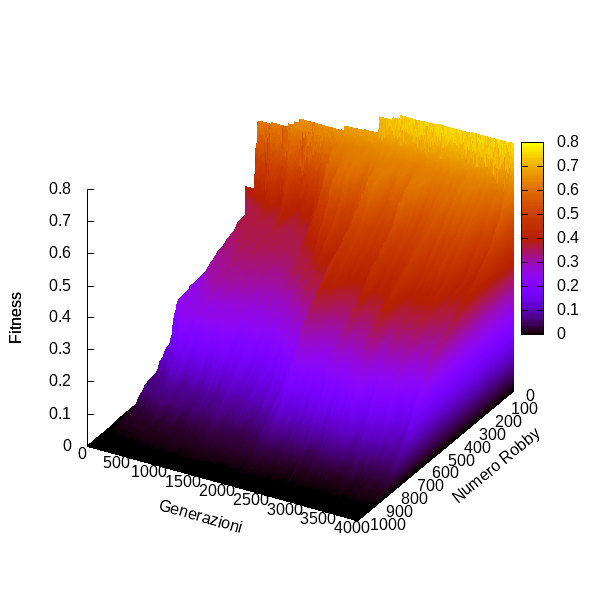
\includegraphics[width=\textwidth]{img/graph10x10.png}
\end{minipage}
\begin{minipage}{.45\textwidth}
	\centering
	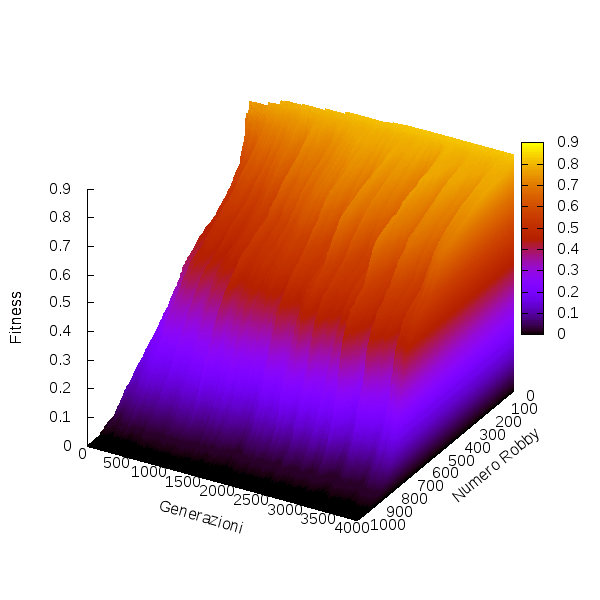
\includegraphics[width=\textwidth]{img/graph5x5.png}
\end{minipage}
\caption{Risultato di 4000 generazioni su mappe di lato 10 (a sinistra) e 5 (a
destra).}
\end{figure}

Come si nota dai grafici, il comportamento dei Robby è quello atteso e la
migliore rete raggiunge valori di fitness di circa $0.8$ corrispondente
all'$80\%$ di lattine raccolte. L'algoritmo è stato inoltre valutato su 100 mappe
non utilizzate nella precedente fase di training. Su mappe di lato 5 ha
raggiunto valori di fitness pari a $0.81$ mentre per mappe di lato 10 valori
pari a $0.78$.  La funzione di fitness sulla mappa più piccola
ha una crescita più rapida che conduce a valori leggermente più alti a causa
del minor spazio di ricerca sulla mappa.\\

Per valutare l'impatto della vista globale presentiamo ora i risultati di 4000
generazioni, su mappe di lato 10 con due Robby:

\begin{figure}[H]
\centering
	\centering
	% XXX: Metti known map!!!
	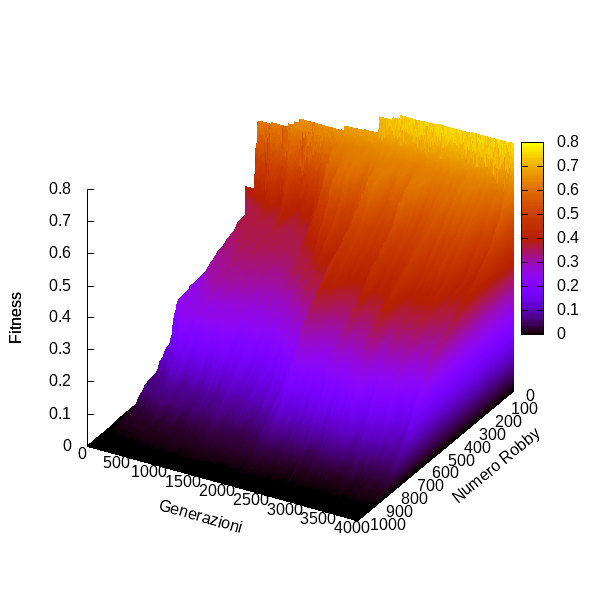
\includegraphics[width=.75\textwidth]{img/graph10x10.png}
\caption{Risultato di 4000 generazioni utilizzando la vista globale su mappe di lato 10.}
\end{figure}

Come facilmente osservabile dal grafico la known map non consente un
apprendimento efficace, specialmente confrontando l'andamento della fitness con
e senza la vista globale.\\

Rispetto ai risultati ottenuti con la vista globale, è lecito chiedersi se sia
possibile implementare un approccio ibrido tra la vista locale con scambio di
messaggi e la vista puramente globale. Questo approccio potrebbe migliorare la
crescita delle reti, consentendo l'algoritmo di superare massimi locali e
\emph{plateau} in modo più efficace. In tal senso un approccio possibile è
l'utilizzo di due insiemi di reti, le une basate su viste locali e le altre su
viste globali. Ciò renderebbe possibile l'utilizzo delle prime per fornire
valori da utilizzare in un apprendimento supervisionato per le seconde. In
alternativa si potrebbe mantenere una memoria di uno storico delle viste locali
precedenti.\\

Un aspetto non trattato in questa relazione è il confronto degli approcci
presentati con l'algoritmo genetico puro. La nozione di posizione, che
risulta di complessa implementazione per l'approccio genetico puro, dovrebbe
condurre a miglioramenti sensibili.
